%% LyX 2.1.4 created this file.  For more info, see http://www.lyx.org/.
%% Do not edit unless you really know what you are doing.
\documentclass[english]{acm_proc_article-sp}
\usepackage[T1]{fontenc}
\setcounter{secnumdepth}{3}
\setcounter{tocdepth}{3}
\usepackage{babel}
\usepackage{float}
\usepackage{multirow}
\usepackage{amstext}
\usepackage{amssymb}
\usepackage{stmaryrd}
\usepackage{graphicx}
\usepackage[unicode=true,pdfusetitle,
 bookmarks=true,bookmarksnumbered=false,bookmarksopen=false,
 breaklinks=false,pdfborder={0 0 1},backref=false,colorlinks=false]
 {hyperref}

\makeatletter

%%%%%%%%%%%%%%%%%%%%%%%%%%%%%% LyX specific LaTeX commands.
%% Because html converters don't know tabularnewline
\providecommand{\tabularnewline}{\\}

%%%%%%%%%%%%%%%%%%%%%%%%%%%%%% User specified LaTeX commands.
\usepackage{etoolbox}
\makeatletter
\def\@copyrightspace{\relax}
\makeatother

\makeatother

\begin{document}

\title{Machine Learning Final Project Report\\
Dropout Prediction in MOOCs}


\author{Chun-Chih Wang, Yi-Lin Cheng, Yih-Chieh Hsu\\
{\normalsize{}Department of Computer Science and Information Engineering,
National Taiwan University}\\
{\small{}\{r04922066, r04922058, r04944001\}@ntu.edu.tw}}
\maketitle
\begin{abstract}
This report describes the solution of \textit{ML or WΓ?} team in NTU
Machine Learning Final Project (Fall, 2015), which aims to predict
the dropouts of online MOOC courses. 
\end{abstract}

\section{Introduction}

We first elaborate our effort on feature engineering and the models
we used. Next, we describe how we used these models combining with
other machine learning methods to improve our performance. Finally,
we present experimental results and discussions among the models.


\section{Feature Engineering }

We keep some of the features provided by TA, and add our own features.
We have spent a lot of time on discovering more useful features. In
the end, we find there are six types of our features performing very
well in the competition in addition to TA's, and there are thirty
dimensions in total of our final features.


\subsection{TA Features}

Among 17 features provided by TA, we remove three features, \textit{chapter\_cnt,
sequential\_cnt }and\textit{ video\_cnt}. In this way, they perform
better when combined with our features.


\subsection{First-Access-Last-Access Difference (day-diff)}

This feature captures the active duration among thirty days, which
can be written as following,

\begin{center}
$\text{day-}\text{diff}=\text{first-access date}-\text{last-access date}$
\par\end{center}

Note that when day-diff is larger, the longer the user is active during
thirty days. Those users with day-diff equal to one, are considered
more likely to drop on the course since they might have a tendency
not to log in in the following ten days.


\subsection{Valid-Video-Log-Count (valid-vlog-cnt)}

We calculate the time differences between those video logs and their
next logs. If they are larger than a minute but smaller than two hours,
then we consider them as valid video events. This shows whether a
user actually watches videos or not.


\subsection{Log-Day-Histogram (log-day)}

We count the number of days each user logged in MOOC within an interval.
We set the interval to seven days to simulate a week. Hence, there
are five weeks in total, with only two days in the last week. By doing
this, we want to capture the behavior of each user through the histogram.


\subsection{Time-Related Features}

Since dropout is defined by whether the user logged in or not in the
following ten days, we think ``time'' is an important indicator.
Therefore, we came up with four time-related features, \textit{First-Access
Difference, Last-Access Difference, Course-Start Difference} and \textit{Course-Access
Difference}. They are all calculated in seconds and divided by 86400
to present in unit of day.


\subsubsection{First-Access Difference (first-access-diff)}

~\\
\centerline{ $\text{first-access-diff}=\text{first-access time}-\min{(\text{first-access time)}}$ }

min(first-access time) is the smallest first-access time among all
users, and the \textit{first-access-diff} of a user is the difference
between the smallest first-access time and the user's first access
time.


\subsubsection{Last-Access Difference (last-access-diff)}

~\\
\centerline{ $\text{last-access-diff}=\text{last-access time}-\min{(\text{last-access time)}}$ }

min(last-access time) is the smallest last-access time among all users,
and the \textit{last-access-diff} of a user is the difference between
the smallest last-access time and the user's last access time.


\subsubsection{Course-Start Difference (course-start-diff)}

~\\
\centerline{ $\text{course-start-diff}=\text{course-start time}-\min{(\text{course-start time)}}$ }

min(course-start time) is the smallest course-start time among all
users, and the \textit{course-start-diff} of a course is the difference
between the smallest course-start time and the course's course-start
time.


\subsubsection{Course-Access Difference (course-access-diff)}

~\\
\centerline{ $\text{course-access-diff}=\text{first-access time}-\min{(\text{course-start time)}}$ }

Calculate the difference between the user's first-access time and
the corresponding course-start time. 


\subsection{Object Count in Course}

We count the number of different objects (discussion, problem, video)
in each course. It is not fair to directly compare the number of logs
among each type of objects. Instead, comparing to the total number
of different objects in a course can bring us more correct results.
Moreover, because there are some missing objects in \textit{object.csv},
we combine all provided files, including \textit{log\_train.csv},
\textit{log\_test.csv},\textit{ object.csv} and count all unique objects
in the same course. Hence, there are three features, \textit{discussion-obj,
problem-obj, video-obj}.


\subsection{Longest Offline/Online Day}

We compute the Longest-Offline-Day (\textit{longest-offline}) and
Longest-Online-Day (\textit{longest-online}). Longest-Offline-Day
is the largest number of days that a user had not logged in continuously,
while Longest-Online-Day is the largest number of days that a user
had logged in continuously. These two features somehow have similar
meanings with \textit{day-diff} but could capture more details of
a user's behavior.


\subsection{Experiment}

Table \ref{feature performance of track 1} and Table \ref{feature performance of track 2}
show how our features performed in this competition. We add each type
of features accumulatively. For example, the third row, ``Before
2.3'' means we use features in Section 2.1, 2.2, 2.3, that is, TA's,
day-diff, valid-vlog-cnt, to verify usefulness of our features. Then,
it is followed by CV, public score and private score of each track.

\begin{table}[h]


\centering{}%
\begin{tabular}{cccc}
\hline 
 & CV & Public & Private\tabularnewline
\hline 
Before 2.1 & 0.948280 & 0.959433 & 0.960796\tabularnewline
Before 2.2 & 0.949790 & 0.958882 & 0.962716\tabularnewline
Before 2.3 & 0.949884 & 0.959281 & 0.962648\tabularnewline
Before 2.4 & 0.950039 & 0.958850 & 0.962304\tabularnewline
Before 2.5 & 0.958273 & 0.967123 & 0.967403\tabularnewline
Before 2.6 & 0.958332 & 0.967588 & 0.967588\tabularnewline
Before 2.7 & 0.958332 & 0.967517 & 0.967158\tabularnewline
\end{tabular}\caption{Evaluation of features in track 1}
\label{feature performance of track 1}
\end{table}


\begin{table}[h]
\centering{}%
\begin{tabular}{cccc}
\hline 
 & CV & Public & Private\tabularnewline
\hline 
Before 2.1 & 0.865182 & 0.875095 & 0.880920\tabularnewline
Before 2.2 & 0.868718 & 0.875326 & 0.881102\tabularnewline
Before 2.3 & 0.869008 & 0.876196 & 0.882107\tabularnewline
Before 2.4 & 0.869880 & 0.875985 & 0.882326\tabularnewline
Before 2.5 & 0.876091 & 0.884886 & 0.888642\tabularnewline
Before 2.6 & 0.876900 & 0.884115 & 0.889476\tabularnewline
Before 2.7 & 0.876931 & 0.883062 & 0.890716\tabularnewline
\end{tabular}\caption{Evaluation of features in track 2}
\label{feature performance of track 2}
\end{table}



\section{Models}

In this section we introduce how we compose our models for dropout
prediction and how we evaluate them. All the following experiments
are running in Python using Scikit-learn \cite{key-2} 1.4. We adopt
5-fold cross-validation to evaluate the performance of each model,
and use different error measures based on different tracks: 
\begin{itemize}
\item Track 1: Average Precision\\
Track 1 uses AP as a metric on ranked list sorted by the probability
estimate that each enrollment would be a dropout. And the score is
based on this formula:
\[
AP(g)=\frac{1}{M}\sum_{n=1}^{M}\frac{dropout_{n}(g)}{n}
\]
,where $dropout_{n}(g)=$ number of dropouts in top n enrollments.\\
According to the above formula, we could realize that what we need
to do is to put the most possible dropout enrollments in front of
non-dropout enrollments (especially in top-M estimates) to maximize
the AP score. 
\item Track 2: Weighted Accuracy\\
Track 2 uses weighted accuracy as a metric based on the result of
binary classification. The basic idea is when one student takes more
courses on the platform, we have more data/information about him/her.
The score is based on this formula:
\[
WA(g)=\frac{\sum_{n=1}^{N}c_{n}^{-1}\left\llbracket g(n^{th}enrollment)=y_{n}\right\rrbracket }{\sum_{n=1}^{N}c_{n}^{-1}}
\]
,where $c_{n}=$ total number of courses the student of the $n^{th}$
enrollment takes.\\
It means that wrong predictions on different enrollments receive different
penalties, hence we assign sample weights in track 2 by the following
approach.
\end{itemize}
Benefited from Scikit-learn, we can easily adopt cross-validation
by its \textit{cross\_validation} module. In all of the models mentioned
in the following section, we set the same scoring metrics and sample
weights based on tracks, where
\begin{itemize}
\item in track 1, we specify \textit{scoring} parameter of \textit{cross\_val\_score}
method to \textit{average\_precision}, and set \textit{sample\_weight}
parameter of \textit{fit} to \textit{None}, indicating all samples
have the same weight.
\item in track 2, we specify \textit{scoring} parameter of \textit{cross\_val\_score}
method to \textit{accuracy}, and set \textit{sample\_weight} parameter
of \textit{fit} to the reciprocal of number of courses of the user
of each enrollment takes.
\end{itemize}

\subsection{Logistic Regression (LR)}

Logistic regression is a common approach that widely used for binary
classification. Based on ``linear first'' principle, we first try
the logistic regression model. Using \textit{LogisticRegression} class
in \textit{linear\_model} module, we could call \textit{predict} and
\textit{predict\_proba} method for track 2 and track 1, respectively,
to get the classification result and the probability estimate. \textit{LogisticRegression
}implements regularized logistic regression using the Liblinear \cite{key-3}
library, where Liblinear solves a L2-regularized unconstrained optimization
problem:

\[
\min_{\mathbf{w}}\frac{1}{2}\mathbf{w}^{\intercal}\mathbf{w}+C\sum_{n=1}^{N}\log\left(1+\exp\left(-y_{n}\mathbf{w^{\intercal}}\mathbf{x}_{n}\right)\right)
\]
,where $C>0$ is a penalty parameter.

By adjusting the $C$ parameter while remaining all other parameters
as default, we get numerical results in Table \ref{result of LR in track1}
by cross-validation.

\begin{table}[h]
\centering{}%
\begin{tabular}{ccc}
\hline 
$C$ & track 1 & track 2\tabularnewline
\hline 
0.01 & \textbf{0.940562} & \textbf{0.858069}\tabularnewline
0.1 & 0.938043 & 0.854190\tabularnewline
1 & 0.938168 & 0.854325\tabularnewline
10 & 0.938227 & 0.854066\tabularnewline
100 & 0.938578 & 0.855061\tabularnewline
\end{tabular}\caption{Performance of Logistic Regression by varying C in track 1 and track
2}
\label{result of LR in track1}
\end{table}



\subsection{Support Vector Machine (SVM)}

Here, we try to exploit support vector machine (SVM) models to solve
the binary classification problem. Given a set of training examples,
each marked one of two categories, an SVM training algorithm builds
a model that assigns new examples into one category or the other,
making it a non-probabilistic binary linear classifier. Because SVM
models only provide the classification results, we only use it in
track 2.


\subsubsection{Linear SVM}

Again, we start from a linear one. Based on \textit{svm} module in
Scikit-learn, we use its \textit{LinearSVC} class as our basic model.
\textit{LinearSVC} is implemented in terms of Liblinear \cite{key-3}. 

Given a set of instance-label pairs $\left(x_{i},y_{i}\right)$, $i=1,2,...,n$
and weights $\mathbf{w}$, Liblinear solves the following unconstrained
optimization problem:

\[
\min_{\mathbf{w}}\frac{1}{2}\mathbf{w}^{\intercal}\mathbf{w}+C\sum_{n=1}^{N}\max\left(1-y_{n}\mathbf{w}^{\intercal}\mathbf{x_{n}},0\right)^{2}
\]
,where $C>0$ is a penalty parameter.

By adjusting the $C$ parameter while remaining all other parameters
as default, we get numerical results in Table \ref{result of liblinear}
by cross-validation.

\begin{table}[h]
\centering{}%
\begin{tabular}{cc}
\hline 
$C$ & track 2\tabularnewline
\hline 
0.01 & 0.864342\tabularnewline
0.1 & 0.864446\tabularnewline
1 & \textbf{0.864550}\tabularnewline
10 & 0.861221\tabularnewline
100 & 0.836313\tabularnewline
\end{tabular}\caption{Performance of linear SVM by varying C }
\label{result of liblinear}
\end{table}



\subsubsection{Non-linear SVM}

We then proceed to use \textit{SVC} class in \textit{svm} module,
which is implemented in terms of LibSVM \cite{key-5}. LibSVM solves
the following optimization problem:

\begin{eqnarray*}
\min_{\mathbf{w,}b,\mathbf{\xi}} &  & \frac{1}{2}\mathbf{w}^{\intercal}\mathbf{w}+C\sum_{n=1}^{N}\xi_{n}\\
\text{subject to } &  & y_{n}\left(\mathbf{w^{\intercal}}\phi\left(\mathbf{x_{n}}\right)+b\right)\geq1-\xi_{n}\\
 &  & \xi_{n}\geq0
\end{eqnarray*}


Here training examples $\mathbf{x_{i}}$ are mapped into a higher
dimensional space by transformation function $\phi$. In our case,
we use the RBF kernel, where

\[
K\left(\mathbf{\mathbf{x_{i}},x_{j}}\right)=\exp\left(-\gamma\left\Vert \mathbf{\mathbf{x_{i}}-x_{j}}\right\Vert ^{2}\right),\ \gamma>0
\]


By adjusting the penalty parameter $C$ and $\gamma$ in RBF kernel
while remaining all other parameters as default, we get numerical
results in Table \ref{result of svm} by cross-validation.

\begin{table}[H]
\centering{}%
\begin{tabular}{cccccc}
\hline 
$C$\textbackslash{}$\gamma$ & 0.01 & 0.1 & 1 & 10 & 100\tabularnewline
\hline 
0.01 & 0.862766 & 0.857498 & 0.793320 & 0.793320 & 0.793320\tabularnewline
0.1 & 0.865877 & 0.865390 & 0.793320 & 0.793320 & 0.793320\tabularnewline
1 & 0.868190 & \textbf{0.868843} & 0.849057 & 0.792946 & 0.793029\tabularnewline
10 & 0.868293 & 0.863036 & 0.840316 & 0.785014 & 0.787886\tabularnewline
100 & 0.866489 & 0.854512 & 0.831190 & 0.777018 & 0.785086\tabularnewline
\end{tabular}\caption{Performance of SVM by varying $C$ and $\gamma$ in track 2}
\label{result of svm}
\end{table}



\subsection{Ensemble Models}

Although the SVM models were popular, they don't provide efficient
computation on large-scale data. We try to use the following ensemble
models to test whether they're effective methods to solve such a classification
problem. The \textit{random\_state} parameters of all of the following
models are set to 1126 for consistency. 


\subsubsection{Random Forest (RF)}

A random forest model is constituted of a number of decision tree
classifiers on various sub-samples of the dataset and use averaging
to improve the predictive accuracy and control over-fitting. The other
mathematical details are ignored here due to space limitation. Using
\textit{RandomForestClassifier} class in \textit{ensemble} module,
we could call \textit{predict} and \textit{predict\_proba} method
for track 2 and track 1, respectively, to get the classification results
and the probability estimates. We control the number of estimators,
which is the number of trees in the forest, and the maximum depth
of the tree to get the following experimental results in Table \ref{result of RF in track1}
and Table \ref{result of RF in track2}.

\begin{table}[H]
\centering{}%
\begin{tabular}{cccc}
\hline 
\#estimators\textbackslash{}max\_depth & 4 & 8 & 12\tabularnewline
\hline 
300 & 0.949010 & 0.954217 & 0.957043\tabularnewline
600 & 0.948916 & 0.954269 & 0.957142\tabularnewline
900 & 0.948960 & 0.954254 & \textbf{0.957145}\tabularnewline
1200 & 0.948970 & 0.954250 & 0.957141\tabularnewline
\end{tabular}\caption{Performance of Random Forest by varying \#estimators and tree depth
in track 1}
\label{result of RF in track1}
\end{table}


\begin{table}[H]
\centering{}%
\begin{tabular}{cccc}
\hline 
\#estimators\textbackslash{}max\_depth & 4 & 8 & 12\tabularnewline
\hline 
300 & 0.866344 & 0.872960 & 0.874515\tabularnewline
600 & 0.866572 & 0.873043 & \textbf{0.874526}\tabularnewline
900 & 0.866727 & 0.873074 & 0.874505\tabularnewline
1200 & 0.866738 & 0.873146 & 0.874411\tabularnewline
\end{tabular}\caption{Performance of Random Forest by varying \#estimators and tree depth
in track 2}
\label{result of RF in track2}
\end{table}



\subsubsection{AdaBoost-Decision Tree (AdaBoost)}

An AdaBoost model fits a classifier on the original dataset and then
fits additional copies of the classifier on the same dataset but the
weights of incorrectly classified instances are adjusted such that
subsequent classifiers focus more on difficult cases. Using \textit{AdaBoostClassifier}
class in \textit{ensemble} module, we could call \textit{predict}
and \textit{predict\_proba} method for track 2 and track 1, respectively,
to get the classification results and the probability estimates. We
control the number of estimators and the maximum depth of base estimator,
where base estimator is decision tree classifier, to get the following
experimental results. Table \ref{result of Ada in track1} shows the
performance in track 1 and track 2.

\begin{table}[H]
\centering{}%
\begin{tabular}{ccc}
\hline 
\#estimators & track 1 & track 2\tabularnewline
\hline 
200 & 0.956061 & 0.872929\tabularnewline
500 & \textbf{0.956378} & 0.87383\tabularnewline
1000 & 0.956151 & \textbf{0.874049}\tabularnewline
2000 & 0.955650 & 0.873852\tabularnewline
\end{tabular}\caption{Performance of AdaBoost-DT by varying \#estimators in track 1 and
track 2}
\label{result of Ada in track1}
\end{table}



\subsubsection{Gradient-Boosted Decision Tree (GBDT)}

A gradient boosted decision tree model builds the model in a stage-wise
fashion, where base learner is decision tree. Using \textit{GradientBoostingClassifier}
class in \textit{ensemble} module, we could call \textit{predict}
and \textit{predict\_proba} method for track 2 and track 1, respectively,
to get the classification results and the probability estimates. We
control the number of estimators and the maximum depth of decision
trees to get the following experimental results in Table \ref{result of GBDT in track1}
and Table \ref{result of GBDT in track2}.

\begin{table}[H]
\centering{}%
\begin{tabular}{cccc}
\hline 
\#estimators\textbackslash{}max\_depth & 2 & 4 & 6\tabularnewline
\hline 
200 & 0.955743 & 0.958041 & 0.958164\tabularnewline
400 & 0.957107 & \textbf{0.958207} & 0.957289\tabularnewline
600 & 0.957636 & 0.958069 & 0.956295\tabularnewline
800 & 0.957892 & 0.957713 & 0.955460\tabularnewline
\end{tabular}\caption{Performance of GBDT by varying \#estimators and tree depth in track
1}
\label{result of GBDT in track1}
\end{table}


\begin{table}[H]
\centering{}%
\begin{tabular}{cccc}
\hline 
\#estimators\textbackslash{}max\_depth & 2 & 4 & 6\tabularnewline
\hline 
200 & 0.873924 & 0.876589 & 0.876890\tabularnewline
400 & 0.875324 & 0.876631 & 0.875168\tabularnewline
600 & 0.875915 & 0.875967 & 0.873872\tabularnewline
800 & 0.876174 & 0.875448 & 0.872638\tabularnewline
\end{tabular}\caption{Performance of GBDT by varying \#estimators and tree depth in track
2}
\label{result of GBDT in track2}
\end{table}



\section{Methods}

Besides using different models for training, we also tried other methods
such as data clustering and model blending to achieve better performance.
Methods we used can be divided into three main categories, which are
\textit{clustering}, \textit{blending} and \textit{Predict track 2
by results of track 1}.

In this section, we are going to explain our implementations of these
three methods. Features used throughout this section are 30-dimension
features presented in Section 2. 


\subsection{Clustering}

Since similar enrollments may have similar behaviors, we grouped them
together and trained each group individually by GBDT. Parameters used
for 5-fold CV were n\_estimators ={[}300,400{]}, max\_depth={[}2,3,4{]},
max\_features={[}``auto'', 0.5{]}\footnote{\textit{max\_features} controls the number of features considered
when looking for the best split. “auto” means max\_features = sqrt(n\_features)
and 0.5 means max\_features = 0.5{*}(n\_features).}. Finally, we combined results from each group together to produce
the final output.


\subsubsection{Cluster by k-means}

There are lots of different clustering algorithms, we chose one of
the most popular algorithms - k-means clustering. Enrollments were
clustered into 3 groups and 5 groups. Results are shown in Table \ref{Cluster by k-means(3 groups)}
and Table \ref{Cluster by k-means(5 groups)}.

\begin{table}[H]
\centering{}%
\begin{tabular}{ccccc}
\hline 
Group ID & \#Train & \#Test & Track 1 CV & Track 2 CV\tabularnewline
\hline 
1 & 24757 & 8687 & 0.951302 & 0.867213\tabularnewline
2 & 46353 & 6381 & 0.965614 & 0.896468\tabularnewline
3 & 25327 & 9040 & 0.945757 & 0.852568\tabularnewline
\end{tabular}\caption{Performance of clustering by k-means (3 groups)}
\label{Cluster by k-means(3 groups)}
\end{table}


\begin{table}[H]
\centering{}%
\begin{tabular}{ccccc}
\hline 
Group ID & \#Train & \#Test & Track 1 CV & Track 2 CV\tabularnewline
\hline 
1 & 25327 & 2714 & 0.945757 & 0.852568\tabularnewline
2 & 11953 & 3411 & 0.962038 & 0.890070\tabularnewline
3 & 15700 & 6961 & 0.969203 & 0.908408\tabularnewline
4 & 24754 & 4641 & 0.951302 & 0.867213\tabularnewline
5 & 18700 & 6381 & 0.963473 & 0.889465\tabularnewline
\end{tabular}\caption{Performance of clustering by k-means (5 groups)}
\label{Cluster by k-means(5 groups)}
\end{table}



\subsubsection{Cluster by day-diff}

Our goal is to predict whether a user will have logs in the 31st-40th
days from the start date of the course. Thus, we considered day-diff
as an important feature. Enrollments were clustered into three groups:
day-diff={[}0,9{]}, day-diff={[}10,19{]}, day-diff={[}20,29{]}. Results
are shown in Table \ref{Cluster by day-diff}. 

\begin{table}[H]
\centering{}%
\begin{tabular}{ccccc}
\hline 
Day-diff & \#Train & \#Test & Track 1 CV & Track 2 CV\tabularnewline
\hline 
0-9 & 25327 & 2714 & 0.945757 & 0.852568\tabularnewline
10-19 & 11953 & 3411 & 0.962038 & 0.890070\tabularnewline
20-29 & 15700 & 6961 & 0.969203 & 0.908408\tabularnewline
\end{tabular}\caption{Performance of clustering by day-diff}
\label{Cluster by day-diff}
\end{table}



\subsubsection{Cluster by Courses}

Since each course has it's own properties, another way to cluster
is dividing enrollments by course ID. There are 39 different courses
in the data set. Due to space limitation, we won't list the CV scores
for each course here. 

The public and private scores of above three clustering approaches
shown in Table \ref{Results of clustering} were not as good as expected.
The results show low accuracy compared to using GBDT to train data
without clustering. One of the reasons may be that after clustering,
number of enrollments in each group was too few. Though the results
are not good enough, they can still be used as sources for blending.

\begin{table}[H]
\centering{}%
\begin{tabular}{ccccc}
\hline 
\multirow{2}{*}{Method} & \multicolumn{2}{c}{track 1} & \multicolumn{2}{c}{track 2}\tabularnewline
\cline{2-5} 
 & Public & Private & Public & Private\tabularnewline
\hline 
GBDT & 0.967417 & 0.967013 & 0.884253 & 0.890386\tabularnewline
K-means (3)  & 0.949614 & 0.949724 & 0.850224 & 0.861440\tabularnewline
K-means (5) & 0.954104 & 0.955305 & 0.848983 & 0.852844\tabularnewline
Day-diff  & 0.965269 & 0.966933 & 0.884276 & 0.888722\tabularnewline
Course & 0.953704 & 0.956637 & 0.879821 & 0.885130\tabularnewline
\end{tabular}\caption{Performance of clustering}
\label{Results of clustering}
\end{table}



\subsection{Blending}

Blending techniques are widely used in machine learning competitions.
By blending outputs from diverse hypotheses, we may obtain more accurate
results.


\subsubsection{Uniform Blending}

Uniform blending can be used in both track 1 and track 2. For track
1, we blended outputs by 

\[
G(\mathbf{x})=\frac{1}{T}\sum_{t=1}^{T}g_{t}(\mathbf{x})
\]


Since different models may output different ranges of probability,
we scaled outputs to {[}0,1{]} by 

\[
y_{i}=\frac{y_{i}-\min_{n\in N}(y_{n})}{\max_{n\in N}(y_{n})-\min_{n\in N(y_{n})}}
\]


before blending. For track 2, we used uniform voting to blend the
outputs. By blending five outputs from Section 4.1, we obtained public/private
score=0.963274/0.964305 for track 1, and public/private score=0.883242/0.889053
for track 2.

We also blended results from three different models: GBDT, RF and
AdaBoost. The results are shown in Table \ref{Results of uniform blending}
below. Parameters used were 
\begin{itemize}
\item GBDT: n\_estimators=400, max\_depth=4, max\_features=0.5 
\item RF: n\_estimators=300, max\_depth=12 
\item AdaBoost: n\_estimators=500
\end{itemize}
\begin{table}[H]
\centering{}%
\begin{tabular}{ccccc}
\hline 
\multirow{2}{*}{Method} & \multicolumn{2}{c}{track 1} & \multicolumn{2}{c}{track 2}\tabularnewline
\cline{2-5} 
 & Public & Private & Public & Private\tabularnewline
\hline 
GBDT & 0.967417 & 0.967013 & 0.884253 & 0.890386\tabularnewline
RF & 0.965330 & 0.967821 & 0.881911 & 0.886911\tabularnewline
AdaBoost & 0.965938 & 0.965091 & 0.879266 & 0.885910\tabularnewline
Uniform Blending & 0.967153 & 0.967423 & 0.883327 & 0.889910\tabularnewline
\end{tabular}\caption{Performance of uniform blending}
\label{Results of uniform blending}
\end{table}



\subsubsection{Stacking (Stacked Generalization)}

Stacking involves training a learning algorithm to combine the predictions
of several other learning algorithms. The original inputs are \textit{training\_data},
\textit{training\_truth}, \textit{testing\_data}. For each single
model, our algorithm involves three steps: 
\begin{enumerate}
\item Partition \textit{training\_data} into five folds: \textit{train\_in\_1},
\textit{}\\
\textit{train\_in\_2}, ... , \textit{train\_in\_5}
\item For i = {[}1,5{]} 

\begin{enumerate}
\item Train $g^{-}$ using four folds other than i-th fold. 
\item Use $g^{-}$ to predict i-th fold and output \textit{train\_out\_i}. 
\item Use $g^{-}$ to predict \textit{testing\_data} (without partitioned)
and output \textit{test\_out\_i}. 
\end{enumerate}
\item Combine \textit{train\_out\_i} into \textit{train\_out}. Take the
mean of \textit{test\_out\_i} to form \textit{test\_out}. 
\end{enumerate}
We used three models: GBDT, RF and AdaBoost for stacking, thus created
three different \textit{train\_out} and \textit{test\_out}. Then,
we ran LR on these three \textit{train\_out }and \textit{test\_out}
to get the final prediction. By using Stacking on track 1, we obtained
public/private score=0.967305/0.967956.


\subsection{Predict Track 2 by Results of Track 1}

A naïve way to convert probability into track 2's 0/1 prediction is
using 0.5 as threshold. Dropout probabilities less than 0.5 are predicted
as 0, otherwise 1. However, we may obtain a better result by finding
a more appropriate threshold. Our approach was to sort track 1's best
result (with the highest public score) together with track 2's best
result by track 1's prediction. We wanted to set the threshold at
point \textit{p} where enrollments were mainly predicted as 0 for
track 2 while track 1's predicted probabilities are less than \textit{p}. 

Our implementation was: 
\begin{enumerate}
\item Define sorted enrollments as $e_{1}$,$e_{2}$,...,$e_{N}$, where
$e_{1}$ has the lowest probability in track 1's prediction. 
\item Change track 2's prediction from 0/1 to -1/+1. 
\item Define $sum_{i}=\sum_{n=1}^{i}$ \{$e_{n}$'s predict value in track
2\}, and $t=\arg\min_{i}sum_{i}$
\item Set threshold \textit{p} = \{$e_{t}$'s predict value in track 1\} 
\end{enumerate}
By setting a more accurate threshold, we improved the performance
from public score=0.884253(threshold=0.5) to public score=0.885174. 


\section{Evaluation}

In this section we evaluate the efficiency, scalability and performance
of each model. Our experiments are conducted on a single machine with
24-core processor and 32GB RAM running Ubuntu 15.04. The code files
and logs are available at our github repository \cite{key-6}.


\subsection{Efficiency}

Table \ref{Efficiency of each model} shows the fitting time of each
model spent on training data. For most models, they spent more time
as N increases, with some strange results. We think these unexpected
results may result from the unstability, or sudden overloading of
our workstation. From Table \ref{Efficiency of each model} , we can
find that linear models, such as linear SVM and LR, cost much less
time compared to other models, while RF and SVM cost most time among
these models. Because SVM needs to construct testing data with RBF
kernel, it costs most predicting time compared to others. ``Paralleled
RF'' means RF paralleled with five cores while ``RF'' is not paralleledd. 

\begin{table}[H]
\centering{}%
\begin{tabular}{ccc}
\hline 
\multirow{1}{*}{Method} & Fitting time (s) & Predicting time (s)\tabularnewline
\hline 
LR & 1.075121 & 0.004284\tabularnewline
Linear SVM & 27.084655 & 0.002636\tabularnewline
SVM & 1242.82098 & 81.870829\tabularnewline
RF & 1116.150098 & 2.638958\tabularnewline
Paralleled RF & 526.611482 & 3.127591\tabularnewline
AdaBoost & 148.405722 & 1.679088\tabularnewline
GBDT & 853.110712 & 0.202299\tabularnewline
\end{tabular}\caption{Efficiency of each model}
\label{Efficiency of each model}
\end{table}



\subsection{Scalability}

We divide all training data into 9 groups, and test the fitting time
of each model with $\frac{N}{9}$, $\frac{2N}{9}$, ..., $N$ enrollments.
The following figures show scalability of each model described in
Section 3. Figure \ref{Figure of efficiency } shows the time each
model spent. Figure \ref{Figure: ratio of time each model spent on each training data}
and Figure \ref{Figure: ratio of time each model spent on each training data (without SVM)}
show the ratio of time each model spent compared to running $\frac{N}{9}$
training data, with SVM and without SVM respectively. SVM has the
poorest scalability compared to other models while logistic regression
has the best scalability. However, paralleled RF has poorer scalability
compared to unparalleled RF. 

\begin{figure}[h]
\begin{centering}
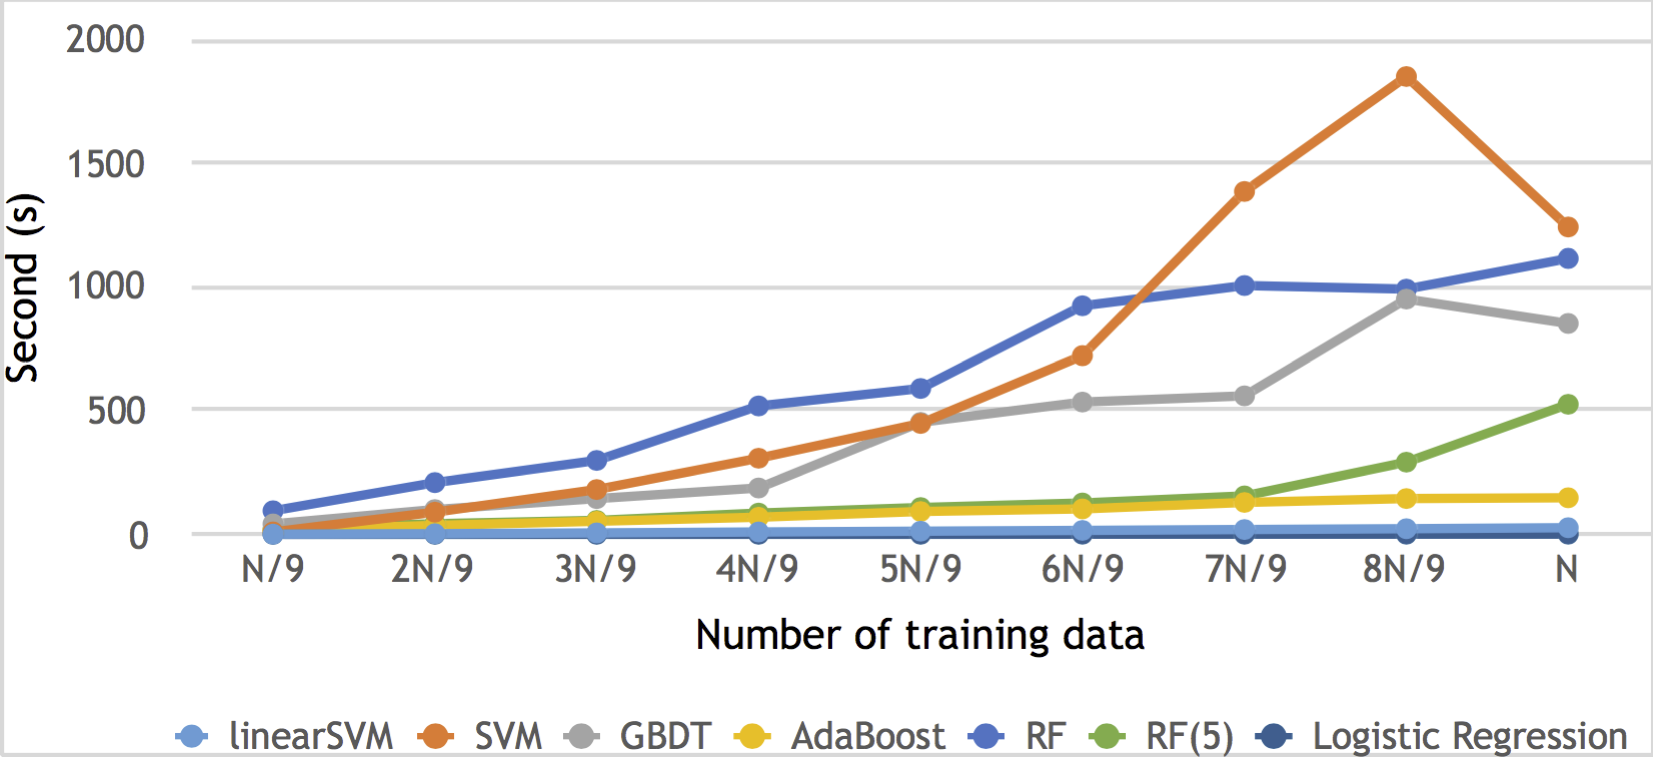
\includegraphics[width=0.8\columnwidth]{figure1}\caption{Running time of each model with different number of training data}

\par\end{centering}

\centering{}\label{Figure of efficiency }
\end{figure}


\begin{figure}[h]
\begin{centering}
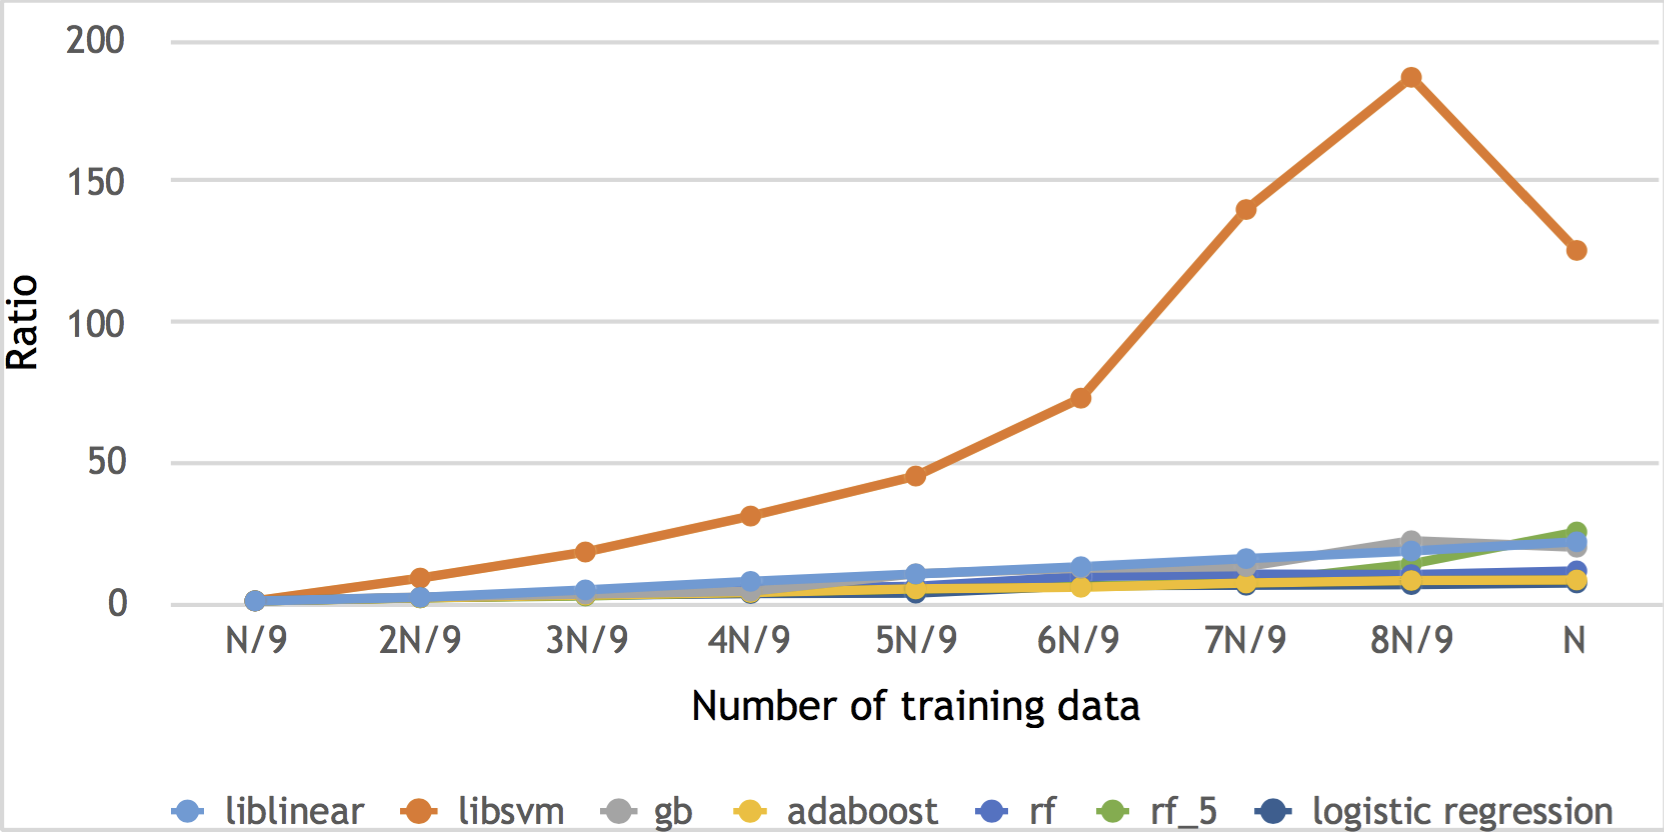
\includegraphics[width=0.8\columnwidth]{figure3}\caption{Ratio of time each model spent with different number of training data}

\par\end{centering}

\centering{}\label{Figure: ratio of time each model spent on each training data}
\end{figure}
\begin{figure}[h]
\begin{centering}
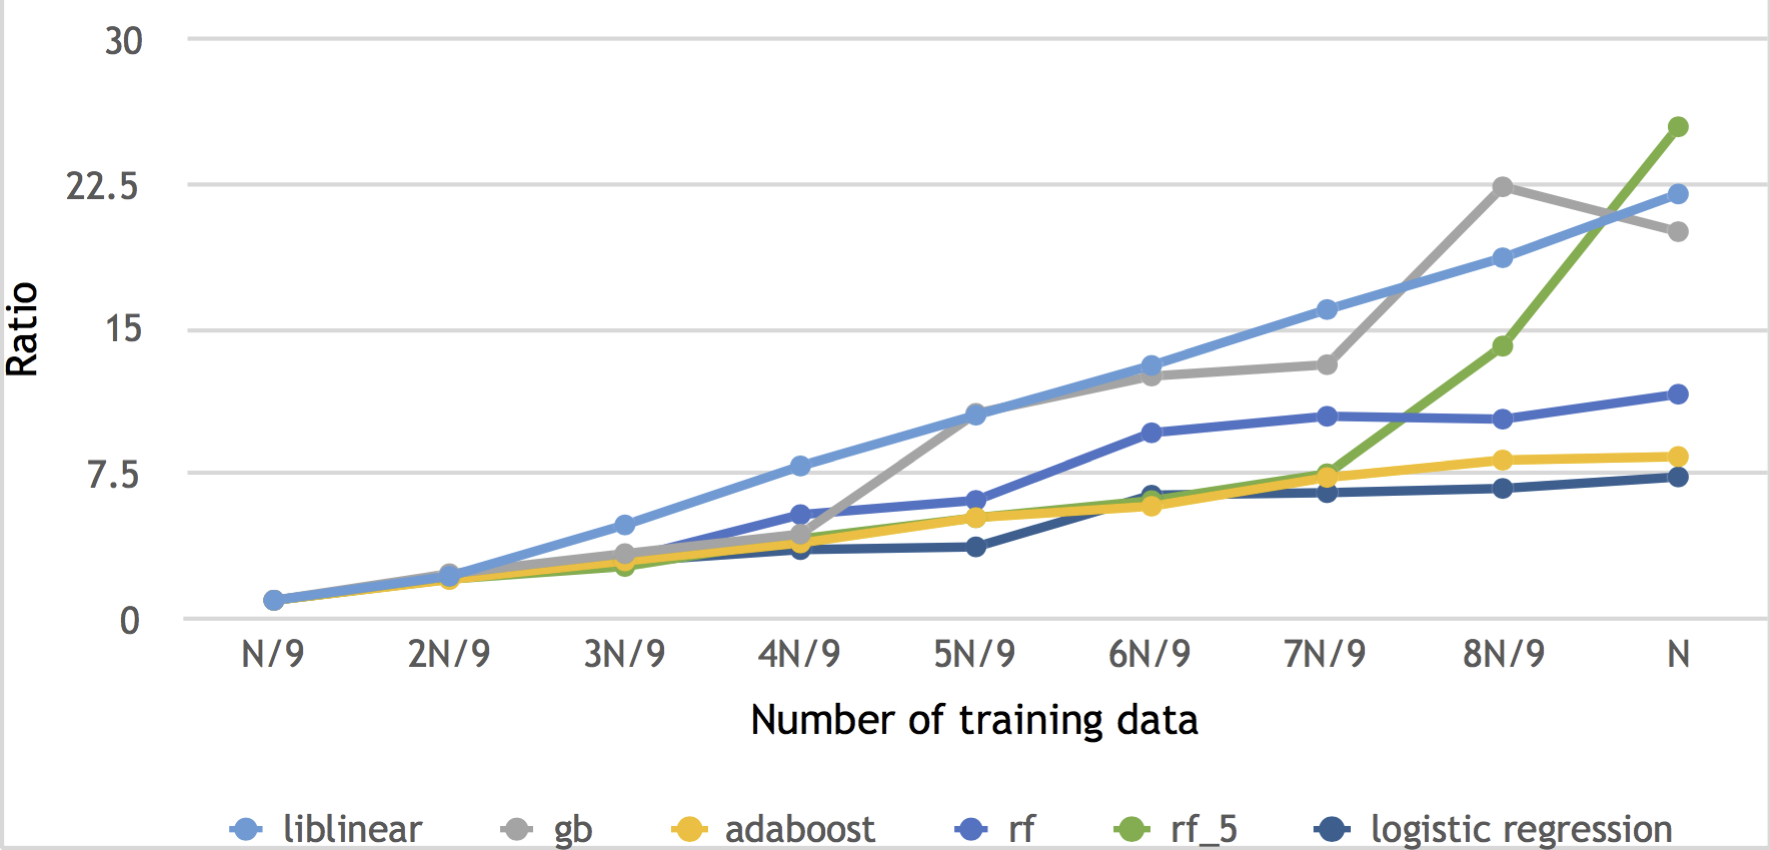
\includegraphics[width=0.8\columnwidth]{figure2}\caption{ratio of time each model spent with different number of training data
(without SVM)}

\par\end{centering}

\centering{}\label{Figure: ratio of time each model spent on each training data (without SVM)}
\end{figure}



\subsection{Performance }

Table \ref{Performance of each model in track 1 and track 2} shows
public score and private score of our models with best parameters
in Section 3. Since SVM and linear SVM can not output probability,
we only evaluate them in track 2. In conclusion, GBDT outperforms
all the other models in public score and private score in track 2.
In this table, we could also find that although linear models cost
less time when fitting training data, their performance are not as
good as the other ones. 

\begin{table}[H]
\centering{}%
\begin{tabular}{ccccc}
\hline 
\multirow{2}{*}{Method} & \multicolumn{2}{c}{track 1} & \multicolumn{2}{c}{track 2}\tabularnewline
\cline{2-5} 
 & Public & Private & Public & Private\tabularnewline
\hline 
LR & 0.942858 & 0.94606 & 0.861871 & 0.871228\tabularnewline
Linear SVM & N/A & N/A & 0.870710 & 0.878081\tabularnewline
SVM & N/A & N/A & 0.877173 & 0.881194\tabularnewline
RF & 0.96482 & 0.967951 & 0.882287 & 0.886508\tabularnewline
AdaBoost & 0.965918 & 0.965125 & 0.879256 & 0.886560\tabularnewline
GBDT & 0.967517 & 0.967517 & 0.884398 & 0.888709\tabularnewline
\end{tabular}\caption{Performance of each model in track 1 and track 2}
\label{Performance of each model in track 1 and track 2}
\end{table}



\section{Conclusion}

We elaborate many useful features in this competition, and compare
the efficiency, scalability, performance between different models.
By applying blending and Stacking methods, we achieve private score
= 0.967723 (rank 18) in track 1 and private score = 0.890957 (rank
8) in track 2 on the final scoreboard.
\begin{thebibliography}{1}
\bibitem{key-2}Scikit-learn: Machine Learning in Python, Pedregosa
et al., JMLR 12, pp. 2825-2830, 2011.

\bibitem{key-3}Rong-En Fan, Kai-Wei Chang, Cho-Jui Hsieh, Xiang-Rui
Wang, and Chih-Jen Lin. 2008. LIBLINEAR: A Library for Large Linear
Classification. J. Mach. Learn. Res. 9 (June 2008), 1871-1874.

\bibitem{key-5}Chih-Chung Chang and Chih-Jen Lin. 2011. LIBSVM: A
library for support vector machines. ACM Trans. Intell. Syst. Technol.
2, 3, Article 27 (May 2011), 27 pages. 

\bibitem{key-6}ML-Final-Project. https://github.com/ylc1218/ML-Final-Project

\bibitem{key-1}\end{thebibliography}

\end{document}
